\chapter{Sparse Kernel Machines}
\label{chap:Sparse Kernel Machines}
\section{Introduction}
One of significant limitations of kernel methods is that the kernel function $\mathcal{k}(\vec{x}_n,\vec{x}_m)$ must be evaluated for all possible pairs $\vec{x}_n$ and $\vec{x}_m$ of training points,computationally infeasible.Kernel-based algorithms that have \textbf{sparse} solutions predict for new inputs depend only on the kernel function evaluated at a subset of the training data points,such as \textbf{suport vector machine}(SVM).
\section{Maximum Margin Classifiers}
Two-class classification problem using linear models
\begin{align}\label{eqn:maximum margin classifier regpresentation}
y(x) = \vec{w}^T\phi(x)+b
\end{align}
where $\phi(x)$ denotes a fixed feature-space transformation,and $b$ is bias parameter.

For linear separable feature space,the parameters satisfies $y(\vec{x}_n)>0$ for points having $t_n=+1$ and $y(\vec{x}_n)<0$ for $t_n=-1$,so that $t_ny(\vec{x}_n)>0$ for all points.

\textbf{Margin} is the smallest distance between the decision boundary and any of the samples.The maximum margin solution can be motivated using \textbf{computational learning theory},also known as \textbf{statistical learning theory}.
\begin{figure*}

	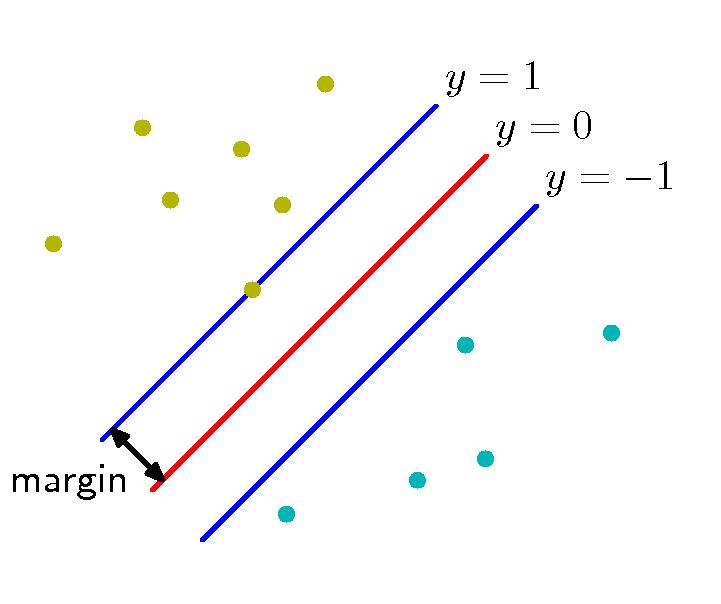
\includegraphics{prml/Figure7.1a.jpg}
	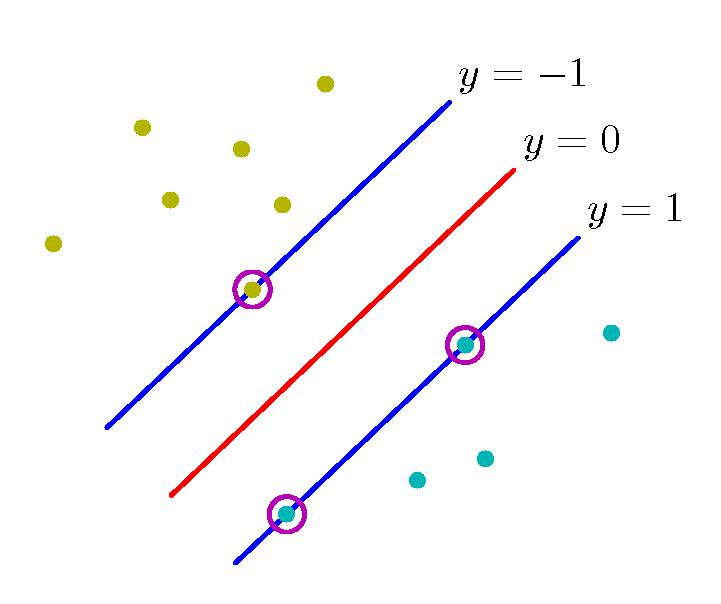
\includegraphics{prml/Figure7.1b.jpg}
	\caption{margin}
\end{figure*}

The \textbf{funtional margin} $t_ny(\vec{x}) > 0$ for data points correctly classified.The maximize it
\begin{align}
\vec{w},b = \arg\max\limits_{\vec{w},b}\{\dfrac{1}{\parallel\vec{w}\parallel}\min_n
[t_n(\vec{w}^T\phi(\vec{x}_n)+b)] \}
\end{align}
We can rescale parameters to set
\begin{align}
t_n(\vec{w}^T\phi(\vec{x}_n)+b) &= 1
\end{align}
for point closet to the surface.Then all data points satisfies the constraint
\begin{align}\label{ineqn:margin constraint}
t_n(\vec{w}^T\phi(\vec{x}_n)+b) \geq 1,n=1,...,N.
\end{align}
This is the \textbf{canonical representation of the decision hyperplane}.The optimization problem is equivalent to
\begin{align}
\arg\min\limits_{\vec{w},b}\dfrac{1}{2}\parallel\vec{w}\parallel^2
\end{align}
subject to constraints \ref{ineqn:margin constraint},which is a \textbf{quadratic programming} problem.

Introducing Lagrange multipliers $a_n\geq 0$
\begin{align}
L(\vec{w},b,\vec{a}) = \dfrac{1}{2}\parallel\vec{w}\parallel^2-
\sum_{n=1}^{N}a_n\{ t_n(\vec{w}^T\phi(\vec{x}_n)+b)-1 \}
\end{align}
where $\vec{a} = (a_1,...,a_N)^T$.Setting the derivatives of $L$ with respect to $\vec{w}$ and $b$ equal to zero,we obtain conditions
\begin{align}
\vec{w}&=\sum_{n=1}^{N}a_n t_n\phi(\vec{x}_n) \\
0 &=\sum_{n=1}^{N}a_n t_n
\end{align}
Eliminating $\vec{w}$ and $b$ gives the \textbf{dual representation} of the maximum margin problem
\begin{align}
\hat{L}(\vec{a})=\sum_{n=1}^{N}a_n -\dfrac{1}{2}\sum_{n=1}^{N}\sum_{m=1}^{N}a_n a_m t_n t_m k(\vec{x}_n,\vec{x}_m)
\end{align}
with respect to $\vec{a}$ subject to the constraints
\begin{align}
a_n &\geq 0,n =1,...,N \\
\sum_{n=1}^{N}a_n t_n &= 0.
\end{align}
The kernel function is defined by $k(\vec{x},\vec{x}') = \phi(\vec{x})^T\phi(\vec{x}')$.

The solution to a quadratic programming problem in $M$ variables has computational complexity of $O(M^3)$.

$y(\vec{x})$ can be expressed by
\begin{align}
y(\vec{x}) = \sum_{n=1}^{N}a_n t_n k(\vec{x},\vec{x}_n) + b.
\end{align}
The $Karush-Kuhn-Tucker(KKT)$ conditions require following the properties hold
\begin{align}
a_n \geq 0 \\
t_n y(\vec{x}_n) -1 &\geq 0 \\
a_n\{t_n y(\vec{x}_n) -1 &= 0\}
\end{align}
Data points for which $a_n=0$ will disappear and remaining ones are called \textbf{suport vectors}.They lie on the maximum margin hyperplanes in feature space.

Having solved the quadratic programming problem,the threshold parameter $b$
\begin{align}
t_n(\sum_{m\in \mathcal{S}}{a_m t_m k(\vec{\vec{x}_n,\vec{x}_m})+b}) =1
\end{align}
where $\mathcal{S}$ denotes the set of indices of the support vectors.Multiply through by $t_n$,making use of $t_n2=1$,and then average these equations over all support vectors
\begin{align}
b=\dfrac{1}{N_{\mathcal{S}}}\sum_{n\in\mathcal{S}}(t_n-\sum_{m\in\mathcal{S}}a_m t_m \mathcal{k}(\vec{x}_n,\vec{x}_m))
\end{align}
where $N_{\mathcal{S}}$ is the total number of support vectors.
Express the maximum-margin classifier in terms of the minimization of an error function with a quadratic regularizer
\begin{align}
\sum_{n=1}^{N}E_{\infty}(y(\vec{x}_n)t_n-1) + \lambda\parallel\vec{w}\parallel^2
\end{align}
where $E_{\infty}(z)$ is zero if $z\geq 0$ and $\infty$ otherwise to ensure the margin constraint.

\subsection{Overlapping class distributions}
In practice,the class-conditional distributions may overlap,in which case exact separation of the training data can lead to poor generalization.Introduce \textbf{slack variables}, $\xi_n\geq 0$ where $n=1,...N$,one for each training data points.We allow points on the 'wrong side' but with a penalty that increases of the distance from the boundary.
\begin{align}
\xi_n = \mid t_n-y(\vec{x}_n)\mid
\end{align}
\begin{SCfigure*}
	\caption{slack variables $\epsilon_n\geq 0$.Data points with circles around them are support vectors}
	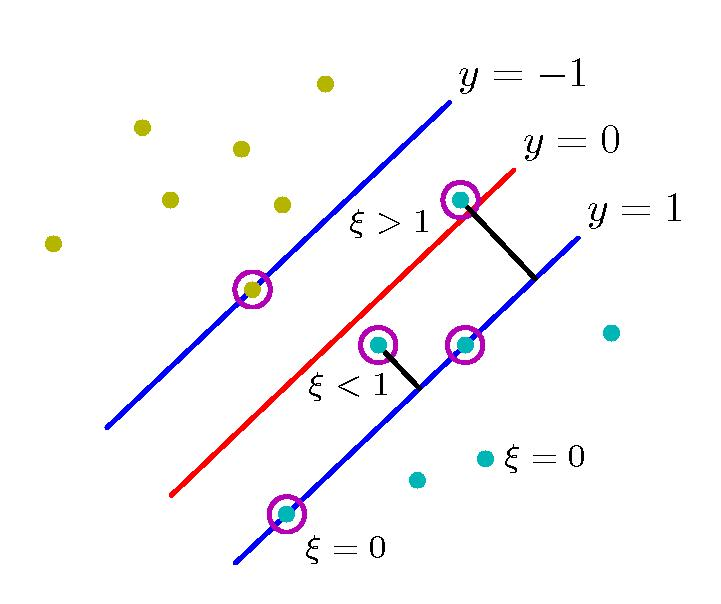
\includegraphics[]{prml/Figure7.3.jpg}
\end{SCfigure*}

Then the classification constraint are replaced by
\begin{align}
t_n y(\vec{x}_n) \geq 1-\xi_n,n=1,...,N
\end{align}
This is described as relaxing the hard margin constraint to give a \textbf{soft margin} and allows misclassification of training set data points.

Maximize the margin with softly penalized points on the wrong side of the margin boundary.
\begin{align}
C\sum_{n=1}^{N}\xi_n +\dfrac{1}{2}\parallel\vec{w}\parallel^2
\end{align}
where the parameter $C$ controls the trade-off between the slack variable penalty and the margin,minimizing errors and controlling model complexity.In the limit $C\longrightarrow \infty$,the model gets more complex,less data points are misclassified.

Minimization with constraint
\begin{align}
L(\vec{w},b\vec{a}) =\dfrac{1}{2}\parallel\vec{w}\parallel^2+C\sum_{n=1}^{N}\xi_n-\sum_{n=1}^{N}a_n\{t_n y(\vec{x}_n)-1+\xi_n \} -\sum_{n=1}^{N}\mu_n\xi_n
\end{align}
where $\{a_n\geq 0\}$ and $\{\mu_n \geq 0 \}$ are Lagrange multipliers.The KKT set of conditions are given by
\begin{align}
a_n &\geq 0 \\
t_n y(\vec{x}_n)-1+\xi_n &\geq 0 \\
a_n(t_n y(\vec{x}_n)-1+\xi_n) &= 0 \\
\mu_n &\geq 0 \\
\xi_n &\geq 0 \\
\mu_n\xi_n &=0
\end{align}
where $n=1,...,N$.

Optimize out $\vec{w},b$ and $\{\xi_n\}$
\begin{align}
\dfrac{\partial L}{\partial\vec{w}} =0 &\Rightarrow \vec{w}=\sum_{n=1}^{N}a_n t_n \\ 
\dfrac{\partial L}{\partial b}=0 &\Rightarrow \sum_{n=1}^{N}a_n t_n =0 \\
\dfrac{\partial L}{\partial \xi_n} =0 &\Rightarrow a_n = C-\mu_n
\end{align}
Eliminated,the dual Lagrangian is in the form
\begin{align}\label{eqn:SVM Lagrangian}
\hat{L}(\vec{a}) = \sum_{n=1}^{N}a_n -\dfrac{1}{2}\sum_{n=1}^{N}\sum_{m=1}^{N}a_n a_m t_n t_m \mathcal{k}(\vec{x}_n,\vec{x}_m)
\end{align}
which is identical to the separable case,with different constraints:
\begin{align}
0\leq a_n \leq C\\
\sum_{n=1}^{N}a_n t_n = 0
\end{align}
for $n=1,...,N$,where the former are known as \textbf{box constraints}.

A subset of data points having $a_n =0$ do not contribute to the predictive model.Support vectors have $a_n > 0$ and satisfy
\begin{align}
t_n y(\vec{x}_n) &= 1-\xi_n
\end{align}
if $a_n <C$,then implies that $\mu_n > 0$,which requires $\xi_n =0$ and hence such points lie on the margin.Points with $a_n=C$ can lie inside the margin and can either be correctly classified if $\xi_n \leq 1$ or misclassified if $\xi_n >1$.

To determine $b$,we note that support vectors for which $0\leq a_n \leq C$ have $\xi_n =0$ so that $t_n y(\vec{x}_n)=1$ and hence satisfy
\begin{align}
t_n(\sum_{m\in\mathcal{S}}a_m t_m \mathcal{k}(\vec{x}_n,\vec{x}_m)+b) =1
\end{align}
A numerically stable solution is obtained by averaging:
\begin{align}
	b=\dfrac{1}{N_{\mathcal{M}}}\sum_{n\in\mathcal{M}} (t_n - \sum_{m\in\mathcal{S}}a_m t_m \mathcal{k}(\vec{x}_n,\vec{x}_m))
\end{align}
where $\mathcal{M}$ denotes the set of indices of data points having $0\leq a_n \leq C$.

\subsubsection{$\nu$-SVM}
Maximize
\begin{align}
\hat{L}(\vec{a})=-\dfrac{1}{2}\sum_{n=1}^{N}\sum_{m=1}^{N}a_n a_m t_n t_m\mathcal{k}(\vec{x}_n,\vec{x}_m)
\end{align}
subject to the constraints
\begin{align}
0\leq a_n \leq 1/N\\
\sum_{n=1}^{N}a_n t_n = 0 \\
\sum_{n=1}^{N}a_n \geq \nu
\end{align}
The parameter $\nu$,which replaces $C$,can be interpreted as both an upper bound on the fraction of \textbf{margin errors} and a lower bound on the fraction of support vectors.

\subsubsection{Optimization}
\begin{description}
	\item[\textbf{chunking}]Lagrangian is unchanged if we remove the rows and columns of the kernel matrix corresponding to Lagrange multipliers.Implemented using \textbf{protected conjugate gradients}.
	\item[\textbf{Decomposition methods}] solves a series of smaller quadratic programming problems but are designed so that each of these is of a fixed size.
	\item[\textbf{sequantial minimal optimization} or SMO] Takes the concept of chunking to the extreme limit and considers just two Lagrange multipliers at a time.Heuristics are given for choosing the pair of Lagrange multipliers to be considered at each step.
\end{description}

Support vector machines don't manage to avoid the curse of dimensionality because there are constraints amongst the feature values that restrict the effective dimensionality of feature space.

\subsubsection{Relation to Logistic Regression}
The objective function can be written 
\begin{align}
\sum_{n=1}^{N}E_{SV}(y_n t_n) +\lambda\parallel\vec{w}\parallel^2
\end{align}
where $\lambda=(2C)^{-1}$,and $E_{SV}(\cdot)$ is the \textbf{hinge} error function defined by
\begin{align}
E_{SV}(y_n t_n)= [1-y_n t_n]_{+}
\end{align}
where $[\cdot]_+$ denotes the positive part.

For logistic regression,target variable $t\in \{-1,1\}$,so
\begin{align}
p(t|y)=\sigma(yt)
\end{align}
Construct an error function by taking the negative logarithm of likelihood function with a quadratic regularizer
\begin{align}
\sum_{n=1}^{N}E_{LR}(y_n t_n)+\lambda\parallel\vec{w}\parallel^2
\end{align}
where
\begin{align}
E_{LR}(yt)=\ln(1+\exp(-yt))
\end{align}
\begin{SCfigure*}
	\caption{Plot of the ‘hinge’ error function used in support vector machines, shown in blue, along with the error function for logistic regression, rescaled by a factor of 1/ ln(2) so that it passes through the point (0, 1), shown in red. Also shown are the misclassification error in black and the squared error in green.}
	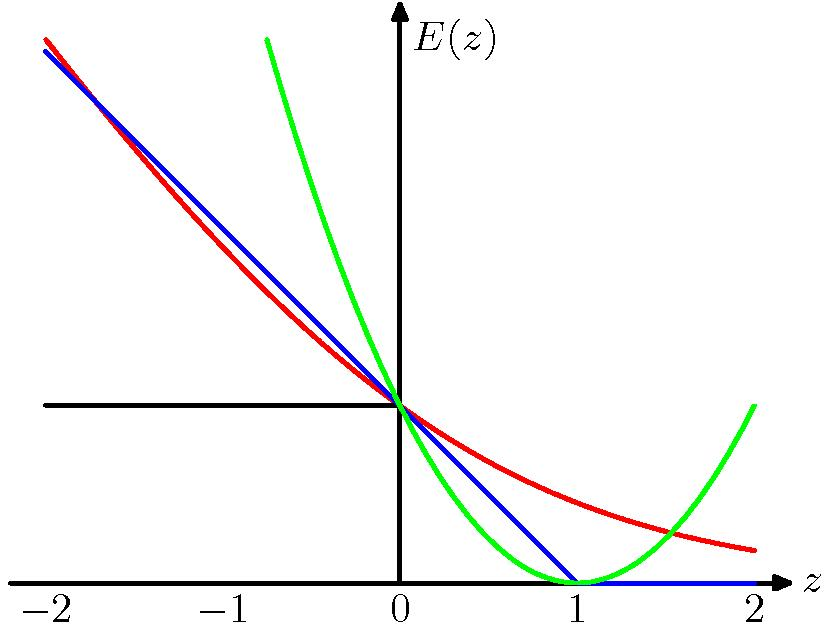
\includegraphics{prml/Figure7.5.jpg}
\end{SCfigure*}

\subsubsection{Multiclass SVMs}
\begin{description}
	\item[\textbf{one-versus-the-rest}] approach:$K$ separate SVMs for each class.
	\item[\textbf{one-versus-one}].$K(K-1)/2$ different 2-class SVMs on possible pairs of classes,which can lead to ambiguities.
	\item[\textbf{single-class}] support vector machines,which solve an unsupervised learning problem related to probability density estimation.
\end{description}

\subsubsection{SVMs for regression}
In simple linear regression we minimize a regularized error function given by
\begin{align}
\dfrac{1}{2}\sum\limits_{n=1}^{N}\{y_n-t_n\}^2+\dfrac{\lambda}{2}\parallel\vec{w}\parallel^2.
\end{align}
To obtain \textbf{sparse solutions},the quadratic error function is replaced by an \textbf{$\epsilon$-insensitive error function}.For example
\begin{align}
E_{\epsilon}(y(\vec{x})-t) = \begin{cases}
0,&\text{if}\mid y(\vec{x})-t\mid < \epsilon;\\
y(\vec{x})-t\mid - \epsilon,&\text{otherwise}
\end{cases}
\end{align}
We therefore minimize
\begin{align}
C\sum\limits_{n=1}^{N}E_{\epsilon}(y(\vec{x}_n)-t_n)+\dfrac{1}{2}\mid\vec{w}\mid^2
\end{align}
where $y(\vec{x})$ is the prediction function.The (inverse) regularization parameter denoted $C$,appears in front of the error term.

Introducing two \textbf{slack variables} for each data point $\vec{x}_n$.The condition for target points to lie inside the $\epsilon$-tube is that $y_n -\epsilon \leq t_n \leq y_n+\epsilon$,and for those outside:
\begin{align}
&\begin{cases}
\xi_n &\geq 0\\
\hat{\xi_n} &\geq 0,n=1,...,N\\
\end{cases}\\
& y(\vec{x}_n)+\epsilon < t_n \leq y(\vec{x}_n)+\epsilon +\xi_n \\
& y(\vec{x}_n)-\epsilon > t_n \geq y(\vec{x}_n)-\epsilon -\hat{\xi_n}
\end{align}
\begin{SCfigure*}
	\caption{Illustration of SVM regression, showing the regression curve together with the $\epsilon$-insensitive tube. }
	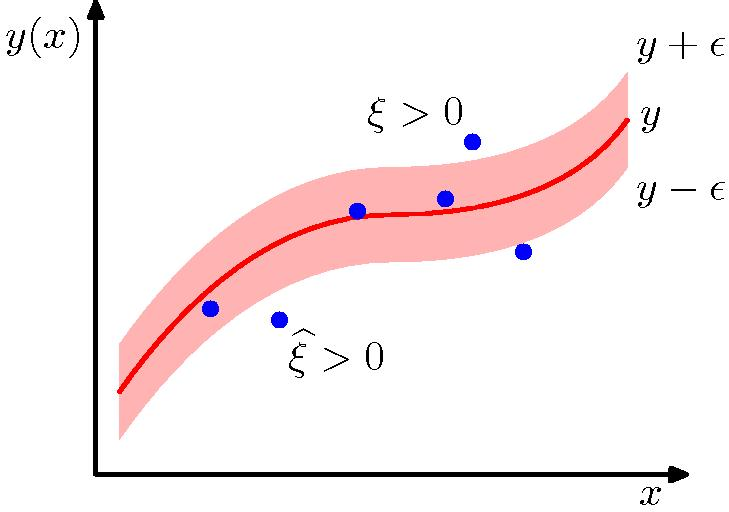
\includegraphics[]{prml/Figure7.7.jpg}
\end{SCfigure*}

The error function for support vector regression can then be written as
\begin{align}
C\sum\limits_{n=1}^{N}(\xi_n+\hat{\xi_n})+\dfrac{1}{2}\parallel\vec{w}\parallel^2
\end{align}
which must be minimized subject to the constraints.Introducing Lagrange multipliers
\begin{align}\label{eqn:svm regression Lagrangian}
L =& C\sum\limits_{n=1}^{N}(\xi_n+\hat{\xi_n})+\dfrac{1}{2}\parallel\vec{w}\parallel^2
- \sum\limits_{n=1}^{N}(\mu_n\xi_n+\hat{\mu_n}\hat{\xi_n}) \\
&-\sum\limits_{n=1}^{N}a_n(\epsilon+\xi_n+y_n-t_n) -\sum\limits_{n=1}^{N}\hat{a_n}(\epsilon+\hat{\xi_n}+y_n-t_n)
\end{align}
Substitute for $y(\vec{x})$ using \ref{eqn:maximum margin classifier regpresentation} and set the derivatives of the Lagrangian with respect to $\vec{x},b,\xi_n,\hat{\xi_n}$ to zero,giving
\begin{align}
\dfrac{\partial L}{\partial\vec{w}} =0 &\Rightarrow \vec{w}=\sum_{n=1}^{N}(a_n-\hat{a_n})\phi(\vec{x}_n) \\
\dfrac{\partial L}{\partial b} =0 &\Rightarrow \sum_{n=1}^{N}(a_n-\hat{a_n})=0 \\
\dfrac{\partial L}{\partial\xi_n} =0 &\Rightarrow a_n+\mu_n=0 \\
\dfrac{\partial L}{\partial\hat{\xi_n}} =0 &\Rightarrow \hat{a_n}+\hat{\mu_n}=0 \\
\end{align}
Using these to eliminate the corresponding variables,we see the dual problem of maximizing 
\begin{align}
\hat{L}(\vec{a},\hat{\vec{a}}) =&-\dfrac{1}{2}\sum_{n=1}^{N}\sum_{m=1}^{N}(a_n-\hat{a_n})(a_m-\hat{a_m})\mathcal{k}(\vec{x}_n,\vec{x}_m) \\
 &-\epsilon\sum_{n=1}^{N}(a_n+\hat{a_n})+\sum_{n=1}^{N}(a_n-\hat{a_n})t_n
\end{align}
with respect to $\{a_n\},\{\hat{a_n}\}	$.We have the \textbf{box constraints}
\begin{align}
0\leq a_n \leq C\\
0\leq \hat{a_n}\leq C
\end{align}
After substitution,the predictions can be made using
\begin{align}
y(\vec{x})=\sum_{n=1}^{N}(a_n-\hat{a_n})\mathcal{k}(\vec{x},\vec{x}_n)+b
\end{align}

The corresponding $karush-Kuhn-Tucker$(KKT) conditons for \ref{eqn:svm regression Lagrangian},which state that \textbf{at the solution the product of the dual variables and the constraints must vanish} are given by
\begin{align}
a_n(\epsilon+\xi_n+y_n-t_n) &= 0\\
\hat{a_n}(\epsilon+\hat{\xi_n}-y_n+t_n) &= 0\\
(C-a_n)\xi_n & = 0\\
(C-\hat{a_n})\hat{\xi_n} &=0
\end{align}

The support vectors are those data points that contribute to predictions,in other words those for which either $a_n \neq 0$ or $\hat{a_n} \neq 0$.These are points lying on the boundary of the $\epsilon$-tube or outside the tube.

The parameter $b$ satisfies 
\begin{align}
\epsilon+y_n-t_n= 0
\end{align}
for points $0<a_n<C$.Solving for it
\begin{align}
b &= t_n-\epsilon-\vec{w}^T\phi(\vec{x}_n) \\
  &= t_n-\epsilon-\sum_{m=1}^{N}(a_m-\hat{a_m})\mathcal{k}(\vec{x}_n,\vec{x}_m)
\end{align}

An alternative formulation of SVM regression is $\nu$ SVM.
\begin{align}
\hat{L}(\vec{a},\hat{\vec{a}}) =&-\dfrac{1}{2}\sum_{n=1}^{N}\sum_{m=1}^{N}(a_n-\hat{a_n})(a_m-\hat{a_m})\mathcal{k}(\vec{x}_n,\vec{x}_m) \\
&-0\times\epsilon\sum_{n=1}^{N}(a_n+\hat{a_n})+\sum_{n=1}^{N}(a_n-\hat{a_n})t_n
\end{align}
subject to constraints
\begin{align}
0\leq a_n &\leq C/N\\
0\leq \hat{a_n} &\leq C/N \\
\sum_{n=1}^{N}(a_n-\hat{a_n}) &=0 \\
\sum_{n=1}^{N}(a_n+\hat{a_n}) &\leq \nu C \\
\end{align}
There are at most $\nu N$ data points falling outside the insensitive tube,which at least $\nu N$ data points are support vectors and so lie either on the tube or outside it.

\section{Relevance Vector Machines}
TODO
where $\mathcal{S}$ denotes the set of indices of the support vectors.

\subsection{Overlapping class distributions}
In practice,the class-conditional distributions may overlap,in which case exact separation of the training data can lead to poor generalization.Introduce \textbf{slack variables}, $\xi_n\geq 0$ where $n=1,...N$,one for each training data points.We allow points on the 'wrong side' but with a penalty that increases of the distance from the boundary.
\begin{align}
\xi_n = \mid t_n-y(\vec{x}_n)\mid
\end{align}
\begin{SCfigure*}
	\caption{slack variables $\epsilon_n\geq 0$.Data points with circles around them are support vectors}
	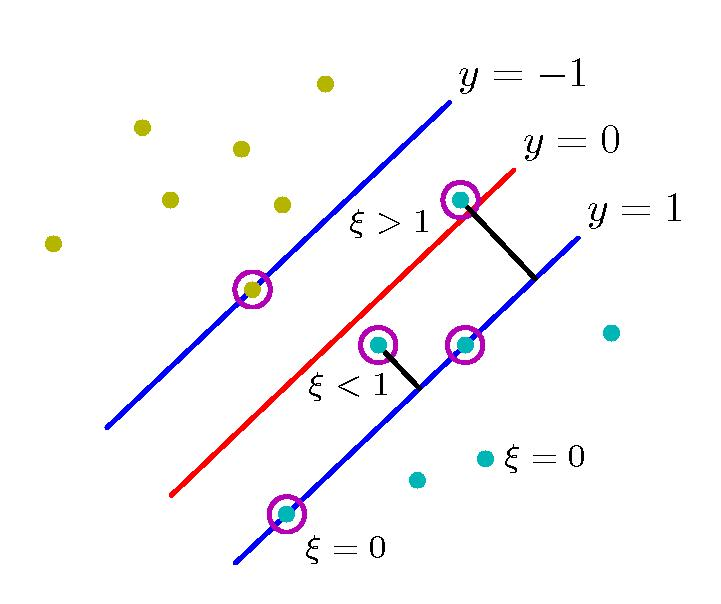
\includegraphics[]{prml/Figure7.3.jpg}
\end{SCfigure*}

Then the classification constraint are replaced by
\begin{align}
t_n y(\vec{x}_n) \geq 1-\epsilon_n,n=1,...,N
\end{align}
This is described as relaxing the hard margin constraint to give a \textbf{soft margin} and allows misclassification of training set data points.

Maximize the margin with softly penalized points on the wrong side of the margin boundary.
\begin{align}
C\sum_{n=1}^{N}\xi_n +\dfrac{1}{2}\parallel\vec{w}\parallel^2
\end{align}
where the parameter $C$ controls the trade-off between the slack variable penalty and the margin,minimizing errors and controlling model complexity.In the limit $C\longrightarrow \infty$,the model gets more complex,less data points are misclassified.

Minimization with constraint
\begin{align}
L(\vec{w},b\vec{a}) =\dfrac{1}{2}\parallel\vec{w}\parallel^2+C\sum_{n=1}^{N}\xi_n-\sum_{n=1}^{N}a_n\{t_n y(\vec{x}_n)-1+\xi_n \} -\sum_{n=1}^{N}\mu_n\xi_n
\end{align}
where $\{a_n\geq 0\}$ and $\{\mu_n \geq 0 \}$ are Lagrange multipliers.The KKT set of conditions are given by
\begin{align}
a_n &\geq 0 \\
t_n y(\vec{x}_n)-1+\xi_n &\geq 0 \\
a_n(t_n y(\vec{x}_n)-1+\xi_n) &= 0 \\
\mu_n &\geq 0 \\
\xi_n &\geq 0 \\
\mu_n\xi_n &=0
\end{align}
where $n=1,...,N$.

Optimize out $\vec{w},b$ and $\{\xi_n\}$
\begin{align}
\dfrac{\partial L}{\partial\vec{w}} &=0 &\Rightarrow \vec{w}=\sum_{n=1}^{N}a_n t_n \\ 
\dfrac{\partial L}{\partial b}&=0 &\Rightarrow \sum_{n=1}^{N}a_n t_n =0 \\
\dfrac{\partial L}{\partial \xi_n} &=0 &\Rightarrow a_n = C-\mu_n
\end{align}
Eliminated,the dual Lagrangian is in the form
\begin{align}\label{eqn:SVM Lagrangian}
\hat{L}(\vec{a}) = \sum_{n=1}^{N}a_n -\dfrac{1}{2}\sum_{n=1}^{N}\sum_{m=1}^{N}a_n a_m t_n t_m \mathcal{k}(\vec{x}_n,\vec{x}_m)
\end{align}
which is identical to the separable case,with different constraints:
\begin{align}
0\leq a_n \leq C\\
\sum_{n=1}^{N}a_n t_n = 0
\end{align}
for $n=1,...,N$,where the former are known as \textbf{box constraints}.

A subset of data points having $a_n =0$ do not contribute to the predictive model.Support vectors have $a_n > 0$ and satisfy
\begin{align}
t_n y(\vec{x}_n) &= 1-\xi_n
\end{align}
if $a_n <C$,then implies that $\mu_n > 0$,which requires $\xi_n =0$ and hence such points lie on the margin.Points with $a_n=C$ can lie inside the margin and can either be correctly classified if $\xi_n \leq 1$ or misclassified if $\xi_n >1$.

To determine $b$,we note that support vectors for which $0\leq a_n \leq C$ have $\xi_n =0$ so that $t_n y(\vec{x}_n)=1$ and hence satisfy
\begin{align}
t_n(\sum_{m\in\mathcal{S}}a_m t_m \mathcal{k}(\vec{x}_n,\vec{x}_m)+b) =1
\end{align}
A numerically stable solution is obtained by averaging:
\begin{align}
	b=\dfrac{1}{N_{\mathcal{M}}}\sum_{n\in\mathcal{M}} (t_n - \sum_{m\in\mathcal{S}}a_m t_m \mathcal{k}(\vec{x}_n,\vec{x}_m))
\end{align}
where $\mathcal{M}$ denotes the set of indices of data points having $0\leq a_n \leq C$.

\subsubsection{$\nu$-SVM}
Maximize
\begin{align}
\hat{L}(\vec{a})=-\dfrac{1}{2}\sum_{n=1}^{N}\sum_{m=1}^{N}a_n a_m t_n t_m\mathcal{k}(\vec{x}_n,\vec{x}_m)
\end{align}
subject to the constraints
\begin{align}
0\leq a_n \leq 1/N\\
\sum_{n=1}^{N}a_n t_n = 0 \\
\sum_{n=1}^{N}a_n \geq \nu
\end{align}







